% ==========================================================================
%  Combined set-up figure: (a) domain, boundary conditions and grid;
%  (b) Edney type IV interaction; (c) grid in the shock layer.
%  
%  Standalone LaTeX document.  On Overleaf: New Project > Blank Project, replace
%  ALL of main.tex with this file (or upload it and set it as the main
%  document) and compile with pdfLaTeX.  In the paper, include the compiled
%  PDF with \includegraphics[width=\textwidth]{...}.
%  
%  Generated by make_figure.py.  Coordinates in mm, origin at the cylinder
%  centre, x downstream, y up.
%  Case: M_inf = 8.03, beta = 18.1 deg -> theta = 12.49 deg, M_2 = 5.252 (gamma = 1.4);
%  R = 38.1 mm, inlet radius 150.39 mm, outlets at phi = +/-65 deg, no-slip wall
%  |phi| <= 45 deg, slip wall beyond, inlet split phi = -12.25 deg.
%  Grid sa_mi_baseline.su2: 294 x 520 cells, polar O-grid, dphi = 0.25 deg,
%  first cell 0.12 um, ratio 1.15 to r = 39.44 mm, uniform 0.20 mm for
%  39.64 <= r <= 75.53 mm, ratio 1.05 to the inlet.  Grid lines shown: (a) every
%  8th ray, (c) every 2nd ray; circles thinned so drawn lines stay apart.
%  Jet: transmitted shock -26.2 deg -> jet direction -15.2 deg, M_jet = 2.40, width 4.5 mm;
%  jet arch, jet bow shock stand-off and shock cells are schematic (solid: compressions, dashed: expansion fans).
% ==========================================================================
\documentclass[border=1pt]{standalone}
% ---- fonts: Helvetica text; sans-serif math (newtxsf) when available
\usepackage[T1]{fontenc}
\usepackage[scaled=0.92]{helvet}
\renewcommand{\familydefault}{\sfdefault}
\IfFileExists{newtxsf.sty}{\usepackage{newtxsf}}{}
\usepackage{tikz}
\usetikzlibrary{arrows.meta}

% ---- colours
\definecolor{ink}{HTML}{111111}
\definecolor{shockgrey}{HTML}{3C3C3C}
\definecolor{dimgrey}{HTML}{7A7A7A}
\definecolor{leadergrey}{HTML}{9A9A9A}
\definecolor{gridgrey}{HTML}{B4B4B4}
\definecolor{bodygrey}{HTML}{E2E2E2}
\definecolor{freeblue}{HTML}{1A5FA8}
\definecolor{postgreen}{HTML}{0E8A62}
\definecolor{slipochre}{HTML}{B06A10}
\definecolor{jetfill}{HTML}{FBEBD3}
\definecolor{accent}{HTML}{C0392B}

% ---- styles
\tikzset{
  lbl/.style={font=\sffamily\small, text=ink, inner sep=1.1pt, align=center},
  sml/.style={font=\sffamily\footnotesize, text=ink, inner sep=1.1pt, align=center},
  halo/.style={fill=white, fill opacity=0.85, text opacity=1},
  region/.style={font=\sffamily\small, text=dimgrey, inner sep=1pt},
  leader/.style={draw=leadergrey, line width=0.4pt},
  freeinlet/.style={draw=freeblue, line width=1.5pt},
  postinlet/.style={draw=postgreen, line width=1.5pt},
  outlet/.style={draw=dimgrey, line width=1.1pt, dash pattern=on 3pt off 2pt, line cap=butt},
  noslip/.style={draw=ink, line width=1.7pt},
  slip/.style={draw=slipochre, line width=1.7pt, dash pattern=on 2pt off 1.1pt, line cap=butt},
  shockA/.style={draw=shockgrey, line width=0.8pt},
  shockB/.style={draw=ink, line width=1.1pt},
  shear/.style={draw=ink, line width=0.7pt, dash pattern=on 2.4pt off 1.4pt, line cap=butt},
  cellshock/.style={draw=ink, line width=0.45pt},
  fan/.style={draw=ink, line width=0.45pt, dash pattern=on 1.4pt off 0.9pt, line cap=butt},
  hatch/.style={draw=dimgrey, line width=0.35pt, line cap=butt},
  flow/.style={line width=0.9pt, -{Stealth[length=2.3mm, width=1.7mm]}},
  jetflow/.style={draw=ink, line width=0.75pt, -{Stealth[length=2mm, width=1.5mm]}},
  dim/.style={draw=dimgrey, line width=0.45pt,
              {Stealth[length=1.5mm, width=1mm]}-{Stealth[length=1.5mm, width=1mm]}},
  triple/.style={circle, fill=ink, inner sep=0pt, minimum size=1.6mm},
  dot/.style={circle, fill=leadergrey, inner sep=0pt, minimum size=1mm},
  panel/.style={font=\sffamily\bfseries\small, inner sep=0pt},
  frame/.style={draw=ink, line width=0.45pt},
  gridA/.style={draw=gridgrey, line width=0.25pt},
  gridC/.style={draw=ink, line width=0.3pt},
  gridedge/.style={draw=ink, line width=0.6pt},
  window/.style={draw=ink, line width=0.5pt, dash pattern=on 1.6pt off 1.1pt, line cap=butt},
  windowC/.style={draw=accent, line width=0.6pt},
}

\begin{document}
\sffamily\small
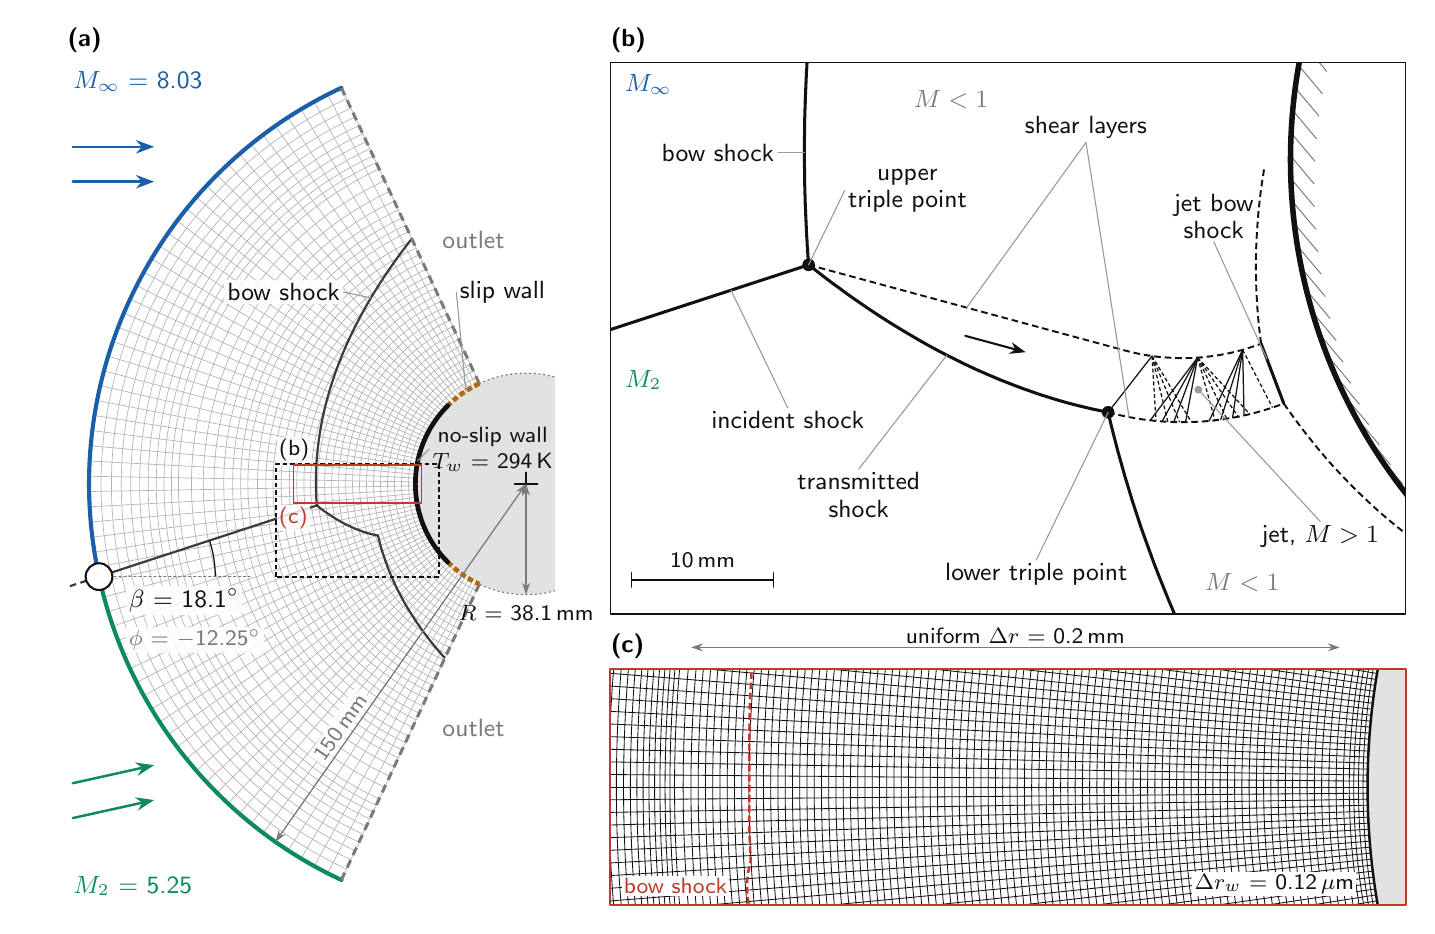
\begin{tikzpicture}[x=1mm, y=1mm, line cap=round, line join=round]

% ======================================================================
%  (a) computational domain, boundary conditions and grid
%      grid: every 8th ray (2 deg); circles thinned to >= 0.85 mm on paper
% ======================================================================
\begin{scope}[shift={(58.31,53.512)}, x=0.36905mm, y=0.36905mm]
  \begin{scope}
    \clip (-158,-145) rectangle (10,145);
    \fill[bodygrey] (0,0) circle[radius=38.1];
    \draw[dimgrey, line width=0.45pt, dash pattern=on 0.4pt off 1.3pt]
      (115:38.1) arc[start angle=115, end angle=-115, radius=38.1];
  \end{scope}

  % grid (41 circles, 66 rays shown)
    \draw[gridA] (115:40.44228) arc[start angle=115, end angle=245, radius=40.44228];
    \draw[gridA] (115:42.8486) arc[start angle=115, end angle=245, radius=42.8486];
    \draw[gridA] (115:45.25491) arc[start angle=115, end angle=245, radius=45.25491];
    \draw[gridA] (115:47.66123) arc[start angle=115, end angle=245, radius=47.66123];
    \draw[gridA] (115:50.06754) arc[start angle=115, end angle=245, radius=50.06754];
    \draw[gridA] (115:52.47386) arc[start angle=115, end angle=245, radius=52.47386];
    \draw[gridA] (115:54.88017) arc[start angle=115, end angle=245, radius=54.88017];
    \draw[gridA] (115:57.28649) arc[start angle=115, end angle=245, radius=57.28649];
    \draw[gridA] (115:59.6928) arc[start angle=115, end angle=245, radius=59.6928];
    \draw[gridA] (115:62.09912) arc[start angle=115, end angle=245, radius=62.09912];
    \draw[gridA] (115:64.50544) arc[start angle=115, end angle=245, radius=64.50544];
    \draw[gridA] (115:66.91175) arc[start angle=115, end angle=245, radius=66.91175];
    \draw[gridA] (115:69.31807) arc[start angle=115, end angle=245, radius=69.31807];
    \draw[gridA] (115:71.72438) arc[start angle=115, end angle=245, radius=71.72438];
    \draw[gridA] (115:74.1307) arc[start angle=115, end angle=245, radius=74.1307];
    \draw[gridA] (115:76.44189) arc[start angle=115, end angle=245, radius=76.44189];
    \draw[gridA] (115:78.88578) arc[start angle=115, end angle=245, radius=78.88578];
    \draw[gridA] (115:81.45773) arc[start angle=115, end angle=245, radius=81.45773];
    \draw[gridA] (115:84.25768) arc[start angle=115, end angle=245, radius=84.25768];
    \draw[gridA] (115:87.04511) arc[start angle=115, end angle=245, radius=87.04511];
    \draw[gridA] (115:89.52326) arc[start angle=115, end angle=245, radius=89.52326];
    \draw[gridA] (115:92.39202) arc[start angle=115, end angle=245, radius=92.39202];
    \draw[gridA] (115:95.71297) arc[start angle=115, end angle=245, radius=95.71297];
    \draw[gridA] (115:98.21291) arc[start angle=115, end angle=245, radius=98.21291];
    \draw[gridA] (115:100.96909) arc[start angle=115, end angle=245, radius=100.96909];
    \draw[gridA] (115:104.00778) arc[start angle=115, end angle=245, radius=104.00778];
    \draw[gridA] (115:107.35794) arc[start angle=115, end angle=245, radius=107.35794];
    \draw[gridA] (115:111.05149) arc[start angle=115, end angle=245, radius=111.05149];
    \draw[gridA] (115:115.12363) arc[start angle=115, end angle=245, radius=115.12363];
    \draw[gridA] (115:119.61316) arc[start angle=115, end angle=245, radius=119.61316];
    \draw[gridA] (115:122.02765) arc[start angle=115, end angle=245, radius=122.02765];
    \draw[gridA] (115:124.56286) arc[start angle=115, end angle=245, radius=124.56286];
    \draw[gridA] (115:127.22484) arc[start angle=115, end angle=245, radius=127.22484];
    \draw[gridA] (115:130.01991) arc[start angle=115, end angle=245, radius=130.01991];
    \draw[gridA] (115:132.95474) arc[start angle=115, end angle=245, radius=132.95474];
    \draw[gridA] (115:136.03631) arc[start angle=115, end angle=245, radius=136.03631];
    \draw[gridA] (115:139.27196) arc[start angle=115, end angle=245, radius=139.27196];
    \draw[gridA] (115:142.6694) arc[start angle=115, end angle=245, radius=142.6694];
    \draw[gridA] (115:146.2367) arc[start angle=115, end angle=245, radius=146.2367];
    \draw[gridA] (115:150.38723) arc[start angle=115, end angle=245, radius=150.38723];
    \draw[gridA] (245:38.1) -- (245:150.3872);
    \draw[gridA] (243:38.1) -- (243:150.3872);
    \draw[gridA] (241:38.1) -- (241:150.3872);
    \draw[gridA] (239:38.1) -- (239:150.3872);
    \draw[gridA] (237:38.1) -- (237:150.3872);
    \draw[gridA] (235:38.1) -- (235:150.3872);
    \draw[gridA] (233:38.1) -- (233:150.3872);
    \draw[gridA] (231:38.1) -- (231:150.3872);
    \draw[gridA] (229:38.1) -- (229:150.3872);
    \draw[gridA] (227:38.1) -- (227:150.3872);
    \draw[gridA] (225:38.1) -- (225:150.3872);
    \draw[gridA] (223:38.1) -- (223:150.3872);
    \draw[gridA] (221:38.1) -- (221:150.3872);
    \draw[gridA] (219:38.1) -- (219:150.3872);
    \draw[gridA] (217:38.1) -- (217:150.3872);
    \draw[gridA] (215:38.1) -- (215:150.3872);
    \draw[gridA] (213:38.1) -- (213:150.3872);
    \draw[gridA] (211:38.1) -- (211:150.3872);
    \draw[gridA] (209:38.1) -- (209:150.3872);
    \draw[gridA] (207:38.1) -- (207:150.3872);
    \draw[gridA] (205:38.1) -- (205:150.3872);
    \draw[gridA] (203:38.1) -- (203:150.3872);
    \draw[gridA] (201:38.1) -- (201:150.3872);
    \draw[gridA] (199:38.1) -- (199:150.3872);
    \draw[gridA] (197:38.1) -- (197:150.3872);
    \draw[gridA] (195:38.1) -- (195:150.3872);
    \draw[gridA] (193:38.1) -- (193:150.3872);
    \draw[gridA] (191:38.1) -- (191:150.3872);
    \draw[gridA] (189:38.1) -- (189:150.3872);
    \draw[gridA] (187:38.1) -- (187:150.3872);
    \draw[gridA] (185:38.1) -- (185:150.3872);
    \draw[gridA] (183:38.1) -- (183:150.3872);
    \draw[gridA] (181:38.1) -- (181:150.3872);
    \draw[gridA] (179:38.1) -- (179:150.3872);
    \draw[gridA] (177:38.1) -- (177:150.3872);
    \draw[gridA] (175:38.1) -- (175:150.3872);
    \draw[gridA] (173:38.1) -- (173:150.3872);
    \draw[gridA] (171:38.1) -- (171:150.3872);
    \draw[gridA] (169:38.1) -- (169:150.3872);
    \draw[gridA] (167:38.1) -- (167:150.3872);
    \draw[gridA] (165:38.1) -- (165:150.3872);
    \draw[gridA] (163:38.1) -- (163:150.3872);
    \draw[gridA] (161:38.1) -- (161:150.3872);
    \draw[gridA] (159:38.1) -- (159:150.3872);
    \draw[gridA] (157:38.1) -- (157:150.3872);
    \draw[gridA] (155:38.1) -- (155:150.3872);
    \draw[gridA] (153:38.1) -- (153:150.3872);
    \draw[gridA] (151:38.1) -- (151:150.3872);
    \draw[gridA] (149:38.1) -- (149:150.3872);
    \draw[gridA] (147:38.1) -- (147:150.3872);
    \draw[gridA] (145:38.1) -- (145:150.3872);
    \draw[gridA] (143:38.1) -- (143:150.3872);
    \draw[gridA] (141:38.1) -- (141:150.3872);
    \draw[gridA] (139:38.1) -- (139:150.3872);
    \draw[gridA] (137:38.1) -- (137:150.3872);
    \draw[gridA] (135:38.1) -- (135:150.3872);
    \draw[gridA] (133:38.1) -- (133:150.3872);
    \draw[gridA] (131:38.1) -- (131:150.3872);
    \draw[gridA] (129:38.1) -- (129:150.3872);
    \draw[gridA] (127:38.1) -- (127:150.3872);
    \draw[gridA] (125:38.1) -- (125:150.3872);
    \draw[gridA] (123:38.1) -- (123:150.3872);
    \draw[gridA] (121:38.1) -- (121:150.3872);
    \draw[gridA] (119:38.1) -- (119:150.3872);
    \draw[gridA] (117:38.1) -- (117:150.3872);
    \draw[gridA] (115:38.1) -- (115:150.3872);

  % shock system (no-field solution)
  \begin{scope}
    \clip (115:150.387) arc[start angle=115, end angle=245, radius=150.387] -- (245:38.1)
      arc[start angle=245, end angle=115, radius=38.1] -- cycle;
    \draw[shockA]
      (-72.03,-7.42) -- (-72.19,-4.94) -- (-72.29,-2.46) -- (-72.33,0.02) -- (-72.31,2.51) --
      (-72.24,4.99) -- (-72.1,7.47) -- (-71.91,9.95) -- (-71.66,12.43) -- (-71.36,14.91) --
      (-70.99,17.39) -- (-70.57,19.87) -- (-70.09,22.35) -- (-69.55,24.83) --
      (-68.96,27.31) -- (-68.3,29.79) -- (-67.59,32.28) -- (-66.82,34.76) -- (-66,37.24) --
      (-65.11,39.72) -- (-64.17,42.2) -- (-63.17,44.68) -- (-62.11,47.16) --
      (-60.99,49.64) -- (-59.82,52.12) -- (-58.59,54.6) -- (-57.3,57.08) -- (-55.96,59.56) --
      (-54.55,62.05) -- (-53.09,64.53) -- (-51.57,67.01) -- (-50,69.49) -- (-48.36,71.97) --
      (-46.67,74.45) -- (-44.93,76.93) -- (-43.12,79.41) -- (-41.26,81.89) --
      (-39.34,84.37) -- (-37.37,86.85) -- (-35.33,89.33) -- (-33.24,91.82) -- (-31.1,94.3) --
      (-28.89,96.78) -- (-26.63,99.26) -- (-24.31,101.74) -- (-21.94,104.22) --
      (-19.51,106.7) -- (-17.02,109.18) -- (-14.48,111.66) -- (-11.88,114.14) --
      (-9.22,116.62) -- (-6.51,119.1) -- (-3.74,121.59) -- (-0.91,124.07) -- (1.97,126.55) --
      (4.91,129.03) -- (7.9,131.51) -- (10.95,133.99) -- (14.05,136.47) -- (17.22,138.95) --
      (20.43,141.43) -- (23.7,143.91) -- (27.03,146.39) -- (30.42,148.87) --
      (33.85,151.36) -- (37.35,153.84) -- (40.9,156.32) -- (44.5,158.8) -- (48.16,161.28) --
      (51.87,163.76) -- (53.75,165);
    \draw[shockA]
      (-50.94,-17.8) -- (-50.36,-20.16) -- (-49.71,-22.5) -- (-48.98,-24.82) --
      (-48.19,-27.13) -- (-47.33,-29.43) -- (-46.39,-31.7) -- (-45.39,-33.97) --
      (-44.32,-36.22) -- (-43.18,-38.45) -- (-41.97,-40.67) -- (-40.69,-42.87) --
      (-39.34,-45.05) -- (-37.92,-47.23) -- (-36.44,-49.38) -- (-34.88,-51.52) --
      (-33.26,-53.65) -- (-31.56,-55.76) -- (-29.8,-57.85) -- (-27.97,-59.93) --
      (-26.07,-62) -- (-24.1,-64.05) -- (-22.06,-66.08) -- (-19.96,-68.1) --
      (-17.79,-70.1) -- (-15.55,-72.09) -- (-13.24,-74.07) -- (-10.86,-76.02) --
      (-8.42,-77.97) -- (-5.91,-79.9) -- (-3.33,-81.81) -- (-0.69,-83.71) -- (2.02,-85.6) --
      (4.79,-87.47) -- (7.64,-89.32) -- (10.54,-91.17) -- (13.52,-92.99) -- (16.56,-94.8) --
      (19.66,-96.6) -- (22.83,-98.38) -- (26.06,-100.15) -- (29.36,-101.91) --
      (32.73,-103.65) -- (36.15,-105.37) -- (39.64,-107.09) -- (43.2,-108.78) --
      (46.82,-110.47) -- (50.5,-112.14) -- (54.24,-113.79) -- (58.05,-115.44) --
      (61.91,-117.07) -- (65.84,-118.68) -- (69.83,-120.28) -- (73.89,-121.87) --
      (78,-123.44) -- (82.18,-125) -- (86.41,-126.55) -- (90.71,-128.08) --
      (95.06,-129.61) -- (99.48,-131.11) -- (103.95,-132.61) -- (108.48,-134.09) --
      (113.07,-135.56) -- (117.72,-137.01) -- (122.43,-138.45) -- (127.2,-139.88) --
      (132.02,-141.3) -- (136.9,-142.71) -- (141.84,-144.1) -- (146.83,-145.48) --
      (149.35,-146.16);
    \draw[shockA]
      (-72.03,-7.42) -- (-70.95,-8.26) -- (-69.87,-9.06) -- (-68.79,-9.84) --
      (-67.71,-10.58) -- (-66.62,-11.29) -- (-65.54,-11.96) -- (-64.46,-12.6) --
      (-63.38,-13.21) -- (-62.3,-13.78) -- (-61.22,-14.32) -- (-60.14,-14.83) --
      (-59.05,-15.3) -- (-57.97,-15.74) -- (-56.89,-16.15) -- (-55.81,-16.53) --
      (-54.73,-16.87) -- (-53.65,-17.18) -- (-52.56,-17.45) -- (-51.48,-17.69) --
      (-50.94,-17.8);
    \draw[shockA] (-146.96,-31.91) -- (-72.03,-7.42);
  \end{scope}
  \draw[shockA, dash pattern=on 2.4pt off 1.6pt, line cap=butt] (-157,-35.19) -- (-146.96,-31.91);

  % boundaries
  \draw[freeinlet] (192.25:150.387) arc[start angle=192.25, end angle=115, radius=150.387];
  \draw[postinlet] (245:150.387) arc[start angle=245, end angle=192.25, radius=150.387];
  \draw[outlet] (115:38.1) -- (115:150.387);
  \draw[outlet] (245:38.1) -- (245:150.387);
  \draw[slip]   (115:38.1) arc[start angle=115, end angle=135, radius=38.1];
  \draw[slip]   (225:38.1) arc[start angle=225, end angle=245, radius=38.1];
  \draw[noslip] (135:38.1) arc[start angle=135, end angle=225, radius=38.1];
  \draw[ink, line width=0.5pt] (-4,0) -- (4,0) (0,-4) -- (0,4);

  % windows of (b) and (c)
  \draw[window] (-86,-32) rectangle (-30,6.83);
  \node[sml, anchor=south west, inner sep=0.8pt, halo] at (-86,6.83) {(b)};
  \draw[windowC] (-80,-6.535) rectangle (-36,6.535);
  \node[sml, text=accent, anchor=north west, inner sep=0.8pt, halo] at (-86,-7.035) {(c)};

  % inlet split and shock angle
  \draw[ink, line width=0.45pt] (-106.96,-31.91) arc[start angle=0, end angle=18.1, radius=40];
  \draw[dimgrey, line width=0.4pt, dash pattern=on 0.8pt off 1pt] (-146.96,-31.91) -- ++(52,0);
  \node[lbl, halo, anchor=north west] at (-137.96,-34.91) {$\beta$ = 18.1$^\circ$};
  \node[sml, halo, text=dimgrey, anchor=north west] at (-137.96,-48.91) {$\phi$ = $-$12.25$^\circ$};
  \filldraw[fill=white, draw=ink, line width=0.75pt] (-146.96,-31.91) circle[radius=4.6];

  % inflow
  \foreach \yy in {116, 104} {\draw[flow, freeblue] (-156,\yy) -- ++(28,0);}
  \node[lbl, text=freeblue, anchor=north west] at (-157,143) {$M_\infty$ = 8.03};
  \foreach \yy in {-103, -115} {\draw[flow, postgreen] (-156,\yy) -- ++(12.49:28.7);}
  \node[lbl, text=postgreen, anchor=south west] at (-157,-143) {$M_2$ = 5.25};

  % boundary labels
  \node[lbl, text=dimgrey, anchor=west] at (-30,84) {outlet};
  \node[lbl, text=dimgrey, anchor=west] at (-30,-84) {outlet};
  \node[lbl, anchor=west] (sw) at (-24,66) {slip wall};
  \draw[leader] (sw.west) -- (-20.75,31.95);
  \node[sml, anchor=center] (ns) at (-11.5,12) {no-slip wall\\$T_w$ = 294\,K};
  \draw[leader] (ns.west) -- (-37.27,7.92);
  \node[lbl, halo, anchor=west] (bs) at (-104,66) {bow shock};
  \draw[leader] (bs.east) -- (-53.41,64);

  % dimensions
  \draw[dim] (0,0) -- (270:38.1);
  \node[sml, anchor=north] at (0,-40.6) {$R$ = 38.1\,mm};
  \draw[dim] (0,0) -- (235:150.387);
  \node[sml, text=dimgrey, halo, rotate=55] at (-63.98,-83.73) {150\,mm};
\end{scope}
\node[panel, anchor=south west] at (0,108.22) {(a)};

% ======================================================================
%  (b) Edney type IV interaction
% ======================================================================
\begin{scope}[shift={(224.107,94.714)}, x=1.80357mm, y=1.80357mm]
  \begin{scope}
    \clip (-86,-32) rectangle (-30,6.825);
    \fill[white] (0,0) circle[radius=38.1];
    \begin{scope}
      \clip (0,0) circle[radius=38.1];
      \draw[hatch] (-24.62,-29.03) -- (-22.82,-31.18);
      \draw[hatch] (-25.82,-27.98) -- (-24.02,-30.13);
      \draw[hatch] (-26.98,-26.88) -- (-25.18,-29.03);
      \draw[hatch] (-28.08,-25.73) -- (-26.28,-27.88);
      \draw[hatch] (-29.14,-24.54) -- (-27.34,-26.69);
      \draw[hatch] (-30.15,-23.3) -- (-28.35,-25.45);
      \draw[hatch] (-31.11,-22.03) -- (-29.31,-24.17);
      \draw[hatch] (-32.01,-20.71) -- (-30.21,-22.85);
      \draw[hatch] (-32.85,-19.36) -- (-31.06,-21.5);
      \draw[hatch] (-33.64,-17.97) -- (-31.84,-20.11);
      \draw[hatch] (-34.37,-16.55) -- (-32.57,-18.69);
      \draw[hatch] (-35.04,-15.1) -- (-33.24,-17.25);
      \draw[hatch] (-35.65,-13.62) -- (-33.85,-15.77);
      \draw[hatch] (-36.2,-12.13) -- (-34.4,-14.27);
      \draw[hatch] (-36.68,-10.6) -- (-34.88,-12.75);
      \draw[hatch] (-37.1,-9.06) -- (-35.3,-11.21);
      \draw[hatch] (-37.45,-7.51) -- (-35.65,-9.65);
      \draw[hatch] (-37.74,-5.94) -- (-35.94,-8.08);
      \draw[hatch] (-37.96,-4.36) -- (-36.16,-6.5);
      \draw[hatch] (-38.12,-2.77) -- (-36.32,-4.91);
      \draw[hatch] (-38.21,-1.18) -- (-36.41,-3.32);
      \draw[hatch] (-38.23,0.42) -- (-36.43,-1.73);
      \draw[hatch] (-38.18,2.01) -- (-36.38,-0.13);
      \draw[hatch] (-38.07,3.61) -- (-36.27,1.46);
      \draw[hatch] (-37.89,5.19) -- (-36.09,3.05);
      \draw[hatch] (-37.65,6.77) -- (-35.85,4.62);
      \draw[hatch] (-37.34,8.33) -- (-35.54,6.19);
      \draw[hatch] (-36.96,9.89) -- (-35.16,7.74);
      \draw[hatch] (-36.52,11.42) -- (-34.72,9.27);
      \draw[hatch] (-36.02,12.93) -- (-34.22,10.79);
      \draw[hatch] (-35.45,14.43) -- (-33.65,12.28);
      \draw[hatch] (-34.83,15.89) -- (-33.03,13.75);
      \draw[hatch] (-34.14,17.33) -- (-32.34,15.19);
      \draw[hatch] (-33.39,18.74) -- (-31.59,16.6);
      \draw[hatch] (-32.58,20.12) -- (-30.78,17.97);
      \draw[hatch] (-31.71,21.46) -- (-29.92,19.31);
      \draw[hatch] (-30.8,22.76) -- (-29,20.62);
      \draw[hatch] (-29.82,24.03) -- (-28.02,21.88);
      \draw[hatch] (-28.8,25.25) -- (-27,23.1);
      \draw[hatch] (-27.72,26.43) -- (-25.92,24.28);
      \draw[hatch] (-26.6,27.56) -- (-24.8,25.42);
      \draw[hatch] (-25.42,28.64) -- (-23.62,26.5);
    \end{scope}
    \draw[noslip, line width=2pt] (135:38.1) arc[start angle=135, end angle=225, radius=38.1];
    \draw[shockB]
      (-72.03,-7.42) -- (-72.05,-7.19) -- (-72.07,-6.96) -- (-72.08,-6.74) --
      (-72.1,-6.51) -- (-72.11,-6.28) -- (-72.13,-6.05) -- (-72.14,-5.83) -- (-72.15,-5.6) --
      (-72.17,-5.37) -- (-72.18,-5.14) -- (-72.19,-4.92) -- (-72.2,-4.69) --
      (-72.21,-4.46) -- (-72.22,-4.23) -- (-72.23,-4.01) -- (-72.24,-3.78) --
      (-72.25,-3.55) -- (-72.26,-3.32) -- (-72.27,-3.1) -- (-72.28,-2.87) --
      (-72.28,-2.64) -- (-72.29,-2.41) -- (-72.29,-2.19) -- (-72.3,-1.96) --
      (-72.31,-1.73) -- (-72.31,-1.5) -- (-72.31,-1.28) -- (-72.32,-1.05) --
      (-72.32,-0.82) -- (-72.32,-0.59) -- (-72.33,-0.37) -- (-72.33,-0.14) --
      (-72.33,0.09) -- (-72.33,0.32) -- (-72.33,0.54) -- (-72.33,0.77) -- (-72.33,1) --
      (-72.33,1.23) -- (-72.33,1.45) -- (-72.32,1.68) -- (-72.32,1.91) -- (-72.32,2.14) --
      (-72.31,2.36) -- (-72.31,2.59) -- (-72.31,2.82) -- (-72.3,3.04) -- (-72.29,3.27) --
      (-72.29,3.5) -- (-72.28,3.73) -- (-72.27,3.95) -- (-72.27,4.18) -- (-72.26,4.41) --
      (-72.25,4.64) -- (-72.24,4.86) -- (-72.23,5.09) -- (-72.22,5.32) -- (-72.21,5.55) --
      (-72.2,5.77) -- (-72.19,6) -- (-72.18,6.23) -- (-72.16,6.46) -- (-72.15,6.68) --
      (-72.14,6.91) -- (-72.12,7.14) -- (-72.11,7.37) -- (-72.1,7.59) -- (-72.08,7.82) --
      (-72.06,8.05) -- (-72.05,8.28) -- (-72.03,8.5) -- (-72.01,8.73) -- (-72,8.96) --
      (-71.98,9.19) -- (-71.96,9.41) -- (-71.94,9.64) -- (-71.92,9.87) -- (-71.9,10.1) --
      (-71.88,10.32) -- (-71.86,10.55) -- (-71.84,10.78) -- (-71.81,11.01) --
      (-71.79,11.23) -- (-71.77,11.46) -- (-71.74,11.69) -- (-71.72,11.92) --
      (-71.7,12.14) -- (-71.67,12.37) -- (-71.65,12.6) -- (-71.62,12.83);
    \draw[shockB]
      (-50.94,-17.8) -- (-50.73,-18.7) -- (-50.5,-19.6) -- (-50.27,-20.5) --
      (-50.02,-21.39) -- (-49.77,-22.28) -- (-49.5,-23.17) -- (-49.23,-24.06) --
      (-48.94,-24.95) -- (-48.65,-25.83) -- (-48.34,-26.71) -- (-48.02,-27.59) --
      (-47.7,-28.47) -- (-47.36,-29.34) -- (-47.01,-30.21) -- (-46.66,-31.08) --
      (-46.29,-31.95) -- (-45.91,-32.81) -- (-45.53,-33.68) -- (-45.13,-34.54) --
      (-44.72,-35.4) -- (-44.3,-36.25) -- (-43.88,-37.11) -- (-43.44,-37.96);
    \draw[shockB] (-90,-13.29) -- (-72.03,-7.42);
    % jet shock cells: compressions (solid), expansion fans (dashed)
    \draw[cellshock] (-50.94,-17.8) -- (-47.85,-13.84);
    \draw[cellshock] (-47.98,-18.37) -- (-44.64,-13.95);
    \draw[cellshock] (-47.15,-18.45) -- (-44.64,-13.95);
    \draw[cellshock] (-46.32,-18.49) -- (-44.64,-13.95);
    \draw[cellshock] (-45.49,-18.5) -- (-44.64,-13.95);
    \draw[cellshock] (-43.83,-18.41) -- (-41.47,-13.4);
    \draw[cellshock] (-43.01,-18.32) -- (-41.47,-13.4);
    \draw[cellshock] (-42.18,-18.19) -- (-41.47,-13.4);
    \draw[cellshock] (-41.37,-18.02) -- (-41.47,-13.4);
    \draw[fan] (-47.85,-13.84) -- (-47.57,-18.41);
    \draw[fan] (-47.85,-13.84) -- (-46.74,-18.47);
    \draw[fan] (-47.85,-13.84) -- (-45.91,-18.5);
    \draw[fan] (-47.85,-13.84) -- (-45.08,-18.49);
    \draw[fan] (-44.64,-13.95) -- (-43.42,-18.37);
    \draw[fan] (-44.64,-13.95) -- (-42.59,-18.26);
    \draw[fan] (-44.64,-13.95) -- (-41.78,-18.11);
    \draw[fan] (-44.64,-13.95) -- (-40.96,-17.93);
    \draw[fan] (-41.47,-13.4) -- (-39.37,-17.47);
    \draw[shockB]
      (-72.03,-7.42) -- (-71.49,-7.84) -- (-70.95,-8.26) -- (-70.41,-8.67) --
      (-69.87,-9.06) -- (-69.33,-9.46) -- (-68.79,-9.84) -- (-68.25,-10.21) --
      (-67.71,-10.58) -- (-67.17,-10.94) -- (-66.62,-11.29) -- (-66.08,-11.63) --
      (-65.54,-11.96) -- (-65,-12.28) -- (-64.46,-12.6) -- (-63.92,-12.91) --
      (-63.38,-13.21) -- (-62.84,-13.5) -- (-62.3,-13.78) -- (-61.76,-14.05) --
      (-61.22,-14.32) -- (-60.68,-14.58) -- (-60.14,-14.83) -- (-59.59,-15.07) --
      (-59.05,-15.3) -- (-58.51,-15.53) -- (-57.97,-15.74) -- (-57.43,-15.95) --
      (-56.89,-16.15) -- (-56.35,-16.34) -- (-55.81,-16.53) -- (-55.27,-16.7) --
      (-54.73,-16.87) -- (-54.19,-17.03) -- (-53.65,-17.18) -- (-53.11,-17.32) --
      (-52.56,-17.45) -- (-52.02,-17.58) -- (-51.48,-17.69) -- (-50.94,-17.8);
    \draw[shear]
      (-72.03,-7.42) -- (-49.65,-13.48) -- (-49.49,-13.52) -- (-49.33,-13.56) --
      (-49.17,-13.6) -- (-49.01,-13.63) -- (-48.85,-13.67) -- (-48.69,-13.7) --
      (-48.53,-13.73) -- (-48.37,-13.76) -- (-48.21,-13.79) -- (-48.05,-13.81) --
      (-47.88,-13.83) -- (-47.72,-13.86) -- (-47.56,-13.88) -- (-47.4,-13.9) --
      (-47.24,-13.91) -- (-47.07,-13.93) -- (-46.91,-13.94) -- (-46.75,-13.95) --
      (-46.58,-13.96) -- (-46.42,-13.97) -- (-46.26,-13.98) -- (-46.09,-13.98) --
      (-45.93,-13.99) -- (-45.77,-13.99) -- (-45.6,-13.99) -- (-45.44,-13.99) --
      (-45.28,-13.98) -- (-45.11,-13.98) -- (-44.95,-13.97) -- (-44.79,-13.96) --
      (-44.62,-13.95) -- (-44.46,-13.94) -- (-44.3,-13.93) -- (-44.14,-13.91) --
      (-43.97,-13.89) -- (-43.81,-13.87) -- (-43.65,-13.85) -- (-43.49,-13.83) --
      (-43.33,-13.81) -- (-43.16,-13.78) -- (-43,-13.75) -- (-42.84,-13.72) --
      (-42.68,-13.69) -- (-42.52,-13.66) -- (-42.36,-13.63) -- (-42.2,-13.59) --
      (-42.04,-13.55) -- (-41.88,-13.51) -- (-41.73,-13.47) -- (-41.57,-13.43) --
      (-41.41,-13.39) -- (-41.25,-13.34) -- (-41.1,-13.29) -- (-40.94,-13.24) --
      (-40.79,-13.19) -- (-40.63,-13.14) -- (-40.48,-13.08) -- (-40.32,-13.03) --
      (-40.17,-12.97);
    \draw[shear]
      (-50.94,-17.8) -- (-50.74,-17.85) -- (-50.53,-17.91) -- (-50.33,-17.96) --
      (-50.12,-18) -- (-49.92,-18.05) -- (-49.71,-18.09) -- (-49.51,-18.13) --
      (-49.3,-18.17) -- (-49.09,-18.21) -- (-48.88,-18.24) -- (-48.67,-18.28) --
      (-48.47,-18.31) -- (-48.26,-18.33) -- (-48.05,-18.36) -- (-47.84,-18.38) --
      (-47.63,-18.41) -- (-47.42,-18.42) -- (-47.21,-18.44) -- (-47,-18.46) --
      (-46.79,-18.47) -- (-46.58,-18.48) -- (-46.37,-18.49) -- (-46.16,-18.49) --
      (-45.94,-18.5) -- (-45.73,-18.5) -- (-45.52,-18.5) -- (-45.31,-18.49) --
      (-45.1,-18.49) -- (-44.89,-18.48) -- (-44.68,-18.47) -- (-44.47,-18.46) --
      (-44.26,-18.45) -- (-44.05,-18.43) -- (-43.84,-18.41) -- (-43.63,-18.39) --
      (-43.42,-18.37) -- (-43.21,-18.34) -- (-43,-18.32) -- (-42.79,-18.29) --
      (-42.58,-18.25) -- (-42.38,-18.22) -- (-42.17,-18.18) -- (-41.96,-18.15) --
      (-41.75,-18.11) -- (-41.55,-18.06) -- (-41.34,-18.02) -- (-41.14,-17.97) --
      (-40.93,-17.92) -- (-40.73,-17.87) -- (-40.52,-17.82) -- (-40.32,-17.76) --
      (-40.12,-17.7) -- (-39.91,-17.64) -- (-39.71,-17.58) -- (-39.51,-17.52) --
      (-39.31,-17.45) -- (-39.11,-17.38) -- (-38.91,-17.31) -- (-38.71,-17.24) --
      (-38.57,-17.19);
    \draw[shear]
      (-40.17,-12.97) -- (-40.33,-11.67) -- (-40.44,-10.37) -- (-40.51,-9.07) --
      (-40.54,-7.78) -- (-40.53,-6.49) -- (-40.47,-5.22) -- (-40.38,-3.95) --
      (-40.25,-2.69) -- (-40.08,-1.45) -- (-39.95,-0.62);
    \draw[shear]
      (-38.57,-17.19) -- (-37.81,-18.26) -- (-37.02,-19.3) -- (-36.21,-20.31) --
      (-35.37,-21.3) -- (-34.5,-22.24) -- (-33.61,-23.16) -- (-32.69,-24.04) --
      (-31.76,-24.89) -- (-30.8,-25.7) -- (-30.15,-26.22);
    \draw[shockB, line width=1.1pt] (-40.17,-12.97) -- (-38.57,-17.19);
  \end{scope}
  \draw[frame] (-86,-32) rectangle (-30,6.825);
  \node[triple] at (-72.03,-7.42) {};
  \node[triple] at (-50.94,-17.8) {};
  \draw[jetflow] (-61,-12.42) -- (-56.75,-13.57);

  % scale bar
  \draw[ink, line width=0.8pt, line cap=butt] (-84.5,-29.6) -- (-74.5,-29.6);
  \draw[ink, line width=0.6pt] (-84.5,-30.1) -- (-84.5,-29.1) (-74.5,-30.1) -- (-74.5,-29.1);
  \node[sml, anchor=south] at (-79.5,-29) {10\,mm};

  % labels
  \node[lbl, text=freeblue, anchor=north west] at (-85.2,6.23) {$M_\infty$};
  \node[lbl, text=postgreen, anchor=north west] at (-85.2,-14.58) {$M_2$};
  \node[lbl, anchor=east] (Lbowshock1) at (-74.2,0.5) {bow shock};
  \draw[leader] (Lbowshock1.east) -- (-72.33,0.5);
  \node[lbl, anchor=west] (Lupper03ext1) at (-69.5,-2.2) {upper\\[-0.3ex]triple point};
  \draw[leader] (Lupper03ext1.west) -- (-72.03,-7.42);
  \node[lbl, anchor=north] (Lincidentsh1) at (-73.5,-17.5) {incident shock};
  \draw[leader] (Lincidentsh1.north) -- (-77.5,-9.2);
  \node[lbl, anchor=north] (Ltransmitte1) at (-68.5,-21.8) {transmitted\\[-0.3ex]shock};
  \draw[leader] (Ltransmitte1.north) -- (-62.3,-13.78);
  \node[lbl, anchor=north] (Llowertripl1) at (-56,-28.2) {lower triple point};
  \draw[leader] (Llowertripl1.north) -- (-50.94,-17.8);
  \node[lbl, anchor=south] (Lshearlayer1) at (-52.5,1.2) {shear layers};
  \draw[leader] (Lshearlayer1.south) -- (-60.9,-10.43);
  \draw[leader] (Lshearlayer1.south) -- (-49.47,-18.14);
  \node[lbl, anchor=south] (Ljetbow03ex1) at (-43.5,-5.8) {jet bow\\[-0.3ex]shock};
  \draw[leader] (Ljetbow03ex1.south) -- (-39.77,-14.03);
  \node[dot] at (-44.59,-16.21) {};
  \node[lbl, anchor=north] (LjetM11) at (-36,-25.5) {jet, $M > 1$};
  \draw[leader] (LjetM11.north) -- (-44.59,-16.21);
  \node[region] at (-62,4.23) {$M < 1$};
  \node[region] at (-41.5,-29.8) {$M < 1$};
\end{scope}
\node[panel, anchor=south west] at (69,108.22) {(b)};

% ======================================================================
%  (c) grid in the shock layer at the stagnation point
%      every 2nd ray (0.5 deg); circles thinned to >= 0.55 mm on paper
% ======================================================================
\begin{scope}[shift={(252.636,15)}, x=2.29545mm, y=2.29545mm]
  \begin{scope}
    \clip (-80,-6.5347) rectangle (-36,6.5347);
    \fill[bodygrey] (0,0) circle[radius=38.1];
    % grid (118 circles, 41 rays shown)
    \draw[gridC] (170:38.34973) arc[start angle=170, end angle=190, radius=38.34973];
    \draw[gridC] (170:38.60312) arc[start angle=170, end angle=190, radius=38.60312];
    \draw[gridC] (170:38.8656) arc[start angle=170, end angle=190, radius=38.8656];
    \draw[gridC] (170:39.11277) arc[start angle=170, end angle=190, radius=39.11277];
    \draw[gridC] (170:39.43965) arc[start angle=170, end angle=190, radius=39.43965];
    \draw[gridC] (170:39.8407) arc[start angle=170, end angle=190, radius=39.8407];
    \draw[gridC] (170:40.24175) arc[start angle=170, end angle=190, radius=40.24175];
    \draw[gridC] (170:40.64281) arc[start angle=170, end angle=190, radius=40.64281];
    \draw[gridC] (170:41.04386) arc[start angle=170, end angle=190, radius=41.04386];
    \draw[gridC] (170:41.44491) arc[start angle=170, end angle=190, radius=41.44491];
    \draw[gridC] (170:41.84596) arc[start angle=170, end angle=190, radius=41.84596];
    \draw[gridC] (170:42.24702) arc[start angle=170, end angle=190, radius=42.24702];
    \draw[gridC] (170:42.64807) arc[start angle=170, end angle=190, radius=42.64807];
    \draw[gridC] (170:43.04912) arc[start angle=170, end angle=190, radius=43.04912];
    \draw[gridC] (170:43.45017) arc[start angle=170, end angle=190, radius=43.45017];
    \draw[gridC] (170:43.85123) arc[start angle=170, end angle=190, radius=43.85123];
    \draw[gridC] (170:44.25228) arc[start angle=170, end angle=190, radius=44.25228];
    \draw[gridC] (170:44.65333) arc[start angle=170, end angle=190, radius=44.65333];
    \draw[gridC] (170:45.05438) arc[start angle=170, end angle=190, radius=45.05438];
    \draw[gridC] (170:45.45544) arc[start angle=170, end angle=190, radius=45.45544];
    \draw[gridC] (170:45.85649) arc[start angle=170, end angle=190, radius=45.85649];
    \draw[gridC] (170:46.25754) arc[start angle=170, end angle=190, radius=46.25754];
    \draw[gridC] (170:46.65859) arc[start angle=170, end angle=190, radius=46.65859];
    \draw[gridC] (170:47.05965) arc[start angle=170, end angle=190, radius=47.05965];
    \draw[gridC] (170:47.4607) arc[start angle=170, end angle=190, radius=47.4607];
    \draw[gridC] (170:47.86175) arc[start angle=170, end angle=190, radius=47.86175];
    \draw[gridC] (170:48.26281) arc[start angle=170, end angle=190, radius=48.26281];
    \draw[gridC] (170:48.66386) arc[start angle=170, end angle=190, radius=48.66386];
    \draw[gridC] (170:49.06491) arc[start angle=170, end angle=190, radius=49.06491];
    \draw[gridC] (170:49.46596) arc[start angle=170, end angle=190, radius=49.46596];
    \draw[gridC] (170:49.86702) arc[start angle=170, end angle=190, radius=49.86702];
    \draw[gridC] (170:50.26807) arc[start angle=170, end angle=190, radius=50.26807];
    \draw[gridC] (170:50.66912) arc[start angle=170, end angle=190, radius=50.66912];
    \draw[gridC] (170:51.07017) arc[start angle=170, end angle=190, radius=51.07017];
    \draw[gridC] (170:51.47123) arc[start angle=170, end angle=190, radius=51.47123];
    \draw[gridC] (170:51.87228) arc[start angle=170, end angle=190, radius=51.87228];
    \draw[gridC] (170:52.27333) arc[start angle=170, end angle=190, radius=52.27333];
    \draw[gridC] (170:52.67438) arc[start angle=170, end angle=190, radius=52.67438];
    \draw[gridC] (170:53.07544) arc[start angle=170, end angle=190, radius=53.07544];
    \draw[gridC] (170:53.47649) arc[start angle=170, end angle=190, radius=53.47649];
    \draw[gridC] (170:53.87754) arc[start angle=170, end angle=190, radius=53.87754];
    \draw[gridC] (170:54.2786) arc[start angle=170, end angle=190, radius=54.2786];
    \draw[gridC] (170:54.67965) arc[start angle=170, end angle=190, radius=54.67965];
    \draw[gridC] (170:55.0807) arc[start angle=170, end angle=190, radius=55.0807];
    \draw[gridC] (170:55.48175) arc[start angle=170, end angle=190, radius=55.48175];
    \draw[gridC] (170:55.8828) arc[start angle=170, end angle=190, radius=55.8828];
    \draw[gridC] (170:56.28386) arc[start angle=170, end angle=190, radius=56.28386];
    \draw[gridC] (170:56.68491) arc[start angle=170, end angle=190, radius=56.68491];
    \draw[gridC] (170:57.08596) arc[start angle=170, end angle=190, radius=57.08596];
    \draw[gridC] (170:57.48702) arc[start angle=170, end angle=190, radius=57.48702];
    \draw[gridC] (170:57.88807) arc[start angle=170, end angle=190, radius=57.88807];
    \draw[gridC] (170:58.28912) arc[start angle=170, end angle=190, radius=58.28912];
    \draw[gridC] (170:58.69017) arc[start angle=170, end angle=190, radius=58.69017];
    \draw[gridC] (170:59.09123) arc[start angle=170, end angle=190, radius=59.09123];
    \draw[gridC] (170:59.49228) arc[start angle=170, end angle=190, radius=59.49228];
    \draw[gridC] (170:59.89333) arc[start angle=170, end angle=190, radius=59.89333];
    \draw[gridC] (170:60.29438) arc[start angle=170, end angle=190, radius=60.29438];
    \draw[gridC] (170:60.69544) arc[start angle=170, end angle=190, radius=60.69544];
    \draw[gridC] (170:61.09649) arc[start angle=170, end angle=190, radius=61.09649];
    \draw[gridC] (170:61.49754) arc[start angle=170, end angle=190, radius=61.49754];
    \draw[gridC] (170:61.8986) arc[start angle=170, end angle=190, radius=61.8986];
    \draw[gridC] (170:62.29965) arc[start angle=170, end angle=190, radius=62.29965];
    \draw[gridC] (170:62.7007) arc[start angle=170, end angle=190, radius=62.7007];
    \draw[gridC] (170:63.10175) arc[start angle=170, end angle=190, radius=63.10175];
    \draw[gridC] (170:63.50281) arc[start angle=170, end angle=190, radius=63.50281];
    \draw[gridC] (170:63.90386) arc[start angle=170, end angle=190, radius=63.90386];
    \draw[gridC] (170:64.30491) arc[start angle=170, end angle=190, radius=64.30491];
    \draw[gridC] (170:64.70596) arc[start angle=170, end angle=190, radius=64.70596];
    \draw[gridC] (170:65.10702) arc[start angle=170, end angle=190, radius=65.10702];
    \draw[gridC] (170:65.50807) arc[start angle=170, end angle=190, radius=65.50807];
    \draw[gridC] (170:65.90912) arc[start angle=170, end angle=190, radius=65.90912];
    \draw[gridC] (170:66.31017) arc[start angle=170, end angle=190, radius=66.31017];
    \draw[gridC] (170:66.71123) arc[start angle=170, end angle=190, radius=66.71123];
    \draw[gridC] (170:67.11228) arc[start angle=170, end angle=190, radius=67.11228];
    \draw[gridC] (170:67.51333) arc[start angle=170, end angle=190, radius=67.51333];
    \draw[gridC] (170:67.91438) arc[start angle=170, end angle=190, radius=67.91438];
    \draw[gridC] (170:68.31544) arc[start angle=170, end angle=190, radius=68.31544];
    \draw[gridC] (170:68.71649) arc[start angle=170, end angle=190, radius=68.71649];
    \draw[gridC] (170:69.11754) arc[start angle=170, end angle=190, radius=69.11754];
    \draw[gridC] (170:69.5186) arc[start angle=170, end angle=190, radius=69.5186];
    \draw[gridC] (170:69.91965) arc[start angle=170, end angle=190, radius=69.91965];
    \draw[gridC] (170:70.3207) arc[start angle=170, end angle=190, radius=70.3207];
    \draw[gridC] (170:70.72175) arc[start angle=170, end angle=190, radius=70.72175];
    \draw[gridC] (170:71.1228) arc[start angle=170, end angle=190, radius=71.1228];
    \draw[gridC] (170:71.52386) arc[start angle=170, end angle=190, radius=71.52386];
    \draw[gridC] (170:71.92491) arc[start angle=170, end angle=190, radius=71.92491];
    \draw[gridC] (170:72.32596) arc[start angle=170, end angle=190, radius=72.32596];
    \draw[gridC] (170:72.72702) arc[start angle=170, end angle=190, radius=72.72702];
    \draw[gridC] (170:73.12807) arc[start angle=170, end angle=190, radius=73.12807];
    \draw[gridC] (170:73.52912) arc[start angle=170, end angle=190, radius=73.52912];
    \draw[gridC] (170:73.93017) arc[start angle=170, end angle=190, radius=73.93017];
    \draw[gridC] (170:74.33123) arc[start angle=170, end angle=190, radius=74.33123];
    \draw[gridC] (170:74.73228) arc[start angle=170, end angle=190, radius=74.73228];
    \draw[gridC] (170:75.13333) arc[start angle=170, end angle=190, radius=75.13333];
    \draw[gridC] (170:75.53438) arc[start angle=170, end angle=190, radius=75.53438];
    \draw[gridC] (170:75.96602) arc[start angle=170, end angle=190, radius=75.96602];
    \draw[gridC] (170:76.44189) arc[start angle=170, end angle=190, radius=76.44189];
    \draw[gridC] (170:76.69782) arc[start angle=170, end angle=190, radius=76.69782];
    \draw[gridC] (170:76.96654) arc[start angle=170, end angle=190, radius=76.96654];
    \draw[gridC] (170:77.24871) arc[start angle=170, end angle=190, radius=77.24871];
    \draw[gridC] (170:77.54497) arc[start angle=170, end angle=190, radius=77.54497];
    \draw[gridC] (170:77.85606) arc[start angle=170, end angle=190, radius=77.85606];
    \draw[gridC] (170:78.18269) arc[start angle=170, end angle=190, radius=78.18269];
    \draw[gridC] (170:78.52566) arc[start angle=170, end angle=190, radius=78.52566];
    \draw[gridC] (170:78.88578) arc[start angle=170, end angle=190, radius=78.88578];
    \draw[gridC] (170:79.2639) arc[start angle=170, end angle=190, radius=79.2639];
    \draw[gridC] (170:79.66093) arc[start angle=170, end angle=190, radius=79.66093];
    \draw[gridC] (170:80.07781) arc[start angle=170, end angle=190, radius=80.07781];
    \draw[gridC] (170:80.51553) arc[start angle=170, end angle=190, radius=80.51553];
    \draw[gridC] (170:80.97514) arc[start angle=170, end angle=190, radius=80.97514];
    \draw[gridC] (170:81.45773) arc[start angle=170, end angle=190, radius=81.45773];
    \draw[gridC] (170:81.96445) arc[start angle=170, end angle=190, radius=81.96445];
    \draw[gridC] (170:82.49651) arc[start angle=170, end angle=190, radius=82.49651];
    \draw[gridC] (170:83.05517) arc[start angle=170, end angle=190, radius=83.05517];
    \draw[gridC] (170:83.64176) arc[start angle=170, end angle=190, radius=83.64176];
    \draw[gridC] (170:84.25768) arc[start angle=170, end angle=190, radius=84.25768];
    \draw[gridC] (170:84.9044) arc[start angle=170, end angle=190, radius=84.9044];
    \draw[gridC] (190:38.1) -- (190:85);
    \draw[gridC] (189.5:38.1) -- (189.5:85);
    \draw[gridC] (189:38.1) -- (189:85);
    \draw[gridC] (188.5:38.1) -- (188.5:85);
    \draw[gridC] (188:38.1) -- (188:85);
    \draw[gridC] (187.5:38.1) -- (187.5:85);
    \draw[gridC] (187:38.1) -- (187:85);
    \draw[gridC] (186.5:38.1) -- (186.5:85);
    \draw[gridC] (186:38.1) -- (186:85);
    \draw[gridC] (185.5:38.1) -- (185.5:85);
    \draw[gridC] (185:38.1) -- (185:85);
    \draw[gridC] (184.5:38.1) -- (184.5:85);
    \draw[gridC] (184:38.1) -- (184:85);
    \draw[gridC] (183.5:38.1) -- (183.5:85);
    \draw[gridC] (183:38.1) -- (183:85);
    \draw[gridC] (182.5:38.1) -- (182.5:85);
    \draw[gridC] (182:38.1) -- (182:85);
    \draw[gridC] (181.5:38.1) -- (181.5:85);
    \draw[gridC] (181:38.1) -- (181:85);
    \draw[gridC] (180.5:38.1) -- (180.5:85);
    \draw[gridC] (180:38.1) -- (180:85);
    \draw[gridC] (179.5:38.1) -- (179.5:85);
    \draw[gridC] (179:38.1) -- (179:85);
    \draw[gridC] (178.5:38.1) -- (178.5:85);
    \draw[gridC] (178:38.1) -- (178:85);
    \draw[gridC] (177.5:38.1) -- (177.5:85);
    \draw[gridC] (177:38.1) -- (177:85);
    \draw[gridC] (176.5:38.1) -- (176.5:85);
    \draw[gridC] (176:38.1) -- (176:85);
    \draw[gridC] (175.5:38.1) -- (175.5:85);
    \draw[gridC] (175:38.1) -- (175:85);
    \draw[gridC] (174.5:38.1) -- (174.5:85);
    \draw[gridC] (174:38.1) -- (174:85);
    \draw[gridC] (173.5:38.1) -- (173.5:85);
    \draw[gridC] (173:38.1) -- (173:85);
    \draw[gridC] (172.5:38.1) -- (172.5:85);
    \draw[gridC] (172:38.1) -- (172:85);
    \draw[gridC] (171.5:38.1) -- (171.5:85);
    \draw[gridC] (171:38.1) -- (171:85);
    \draw[gridC] (170.5:38.1) -- (170.5:85);
    \draw[gridC] (170:38.1) -- (170:85);
    \draw[gridedge, line width=0.9pt] (170:38.1) arc[start angle=170, end angle=190, radius=38.1];
    % no-field bow shock
    \draw[accent, line width=0.9pt, dash pattern=on 2.4pt off 1.3pt, line cap=butt]
      (-66.25,36.26) -- (-67.22,33.51) -- (-68.11,30.68) -- (-68.89,27.84) --
      (-69.7,24.34) -- (-70.81,18.31) -- (-71.25,15.47) -- (-71.45,13.89) --
      (-71.71,11.68) -- (-72.15,6.95) -- (-72.27,4.74) -- (-72.31,2.52) -- (-72.3,-2.52) --
      (-72.23,-4.1) -- (-72.38,-4.74) -- (-72.44,-5.38) -- (-72.41,-6.02) -- (-72.3,-6.64) --
      (-72.1,-7.26) -- (-71.81,-7.87) -- (-71.43,-8.45) -- (-70.97,-9.03) --
      (-70.42,-9.58) -- (-69.79,-10.12) -- (-69.44,-10.38) -- (-67.54,-11.3) --
      (-65.63,-12.16) -- (-63.7,-12.96) -- (-61.78,-13.7) -- (-59.84,-14.37) --
      (-54.49,-16.14) -- (-53.42,-16.59) -- (-52.8,-16.9) -- (-52.27,-17.24) --
      (-51.82,-17.59) -- (-51.45,-17.97) -- (-51.14,-18.36) -- (-50.76,-18.98) --
      (-50.57,-19.41) -- (-50.3,-20.32) -- (-49.19,-24.26) -- (-48.66,-25.87) --
      (-48.07,-27.47) -- (-47.34,-29.29) -- (-44.66,-35.53) -- (-44.39,-36.09);
  \end{scope}
  \draw[windowC, line width=0.7pt] (-80,-6.5347) rectangle (-36,6.5347);

  % uniform-spacing band
  \draw[dim] (-75.53,7.735) -- (-39.64,7.735);
  \node[sml, anchor=south, fill=white, inner sep=0.6pt] at (-57.59,7.835)
    {uniform $\Delta r$ = 0.2\,mm};
  \node[sml, text=accent, anchor=south west, fill=white, inner sep=0.8pt] at (-79.4,-6.035)
    {bow shock};
  \node[sml, anchor=south east, fill=white, inner sep=0.8pt] at (-38.7,-6.035)
    {$\Delta r_w$ = 0.12\,$\mu$m};
\end{scope}
\node[panel, anchor=south west] at (69,31.2) {(c)};
\end{tikzpicture}
\end{document}
